\documentclass[landscape,footrule]{foils}
\usepackage[lecture-serie]{foiltex-extra}
\usepackage{crysymb}
\usepackage{graphics}
\usepackage[pdftex]{graphicx} 




\newcommand{\lecture}{Basics of probabilistic modelling}
\newcommand{\lserie}{LTAT.02.004 Machine Learning II}
\newcommand{\ldate}{February 25, 2019}
\newcommand{\lauthor}{Sven Laur}
\newcommand{\linst}{University of Tartu}
\graphicspath{{./illustrations/}}


\newcommand{\leqm}{\ \leq_m}


\newcommand{\bigvskip}{\vskip 2em}
\newcommand{\lastline}{\vspace*{-2ex}}
\newcommand{\spreadappart}{\vspace*{\fill}}

\DeclareMathOperator{\supp}{supp}
\DeclareMathOperator{\conf}{conf}
\DeclareMathOperator{\precision}{precision}
\DeclareMathOperator{\recall}{recall}


\begin{document}
\titlefoil

\foilhead[-0cm]{What is probability?}

\begin{center}
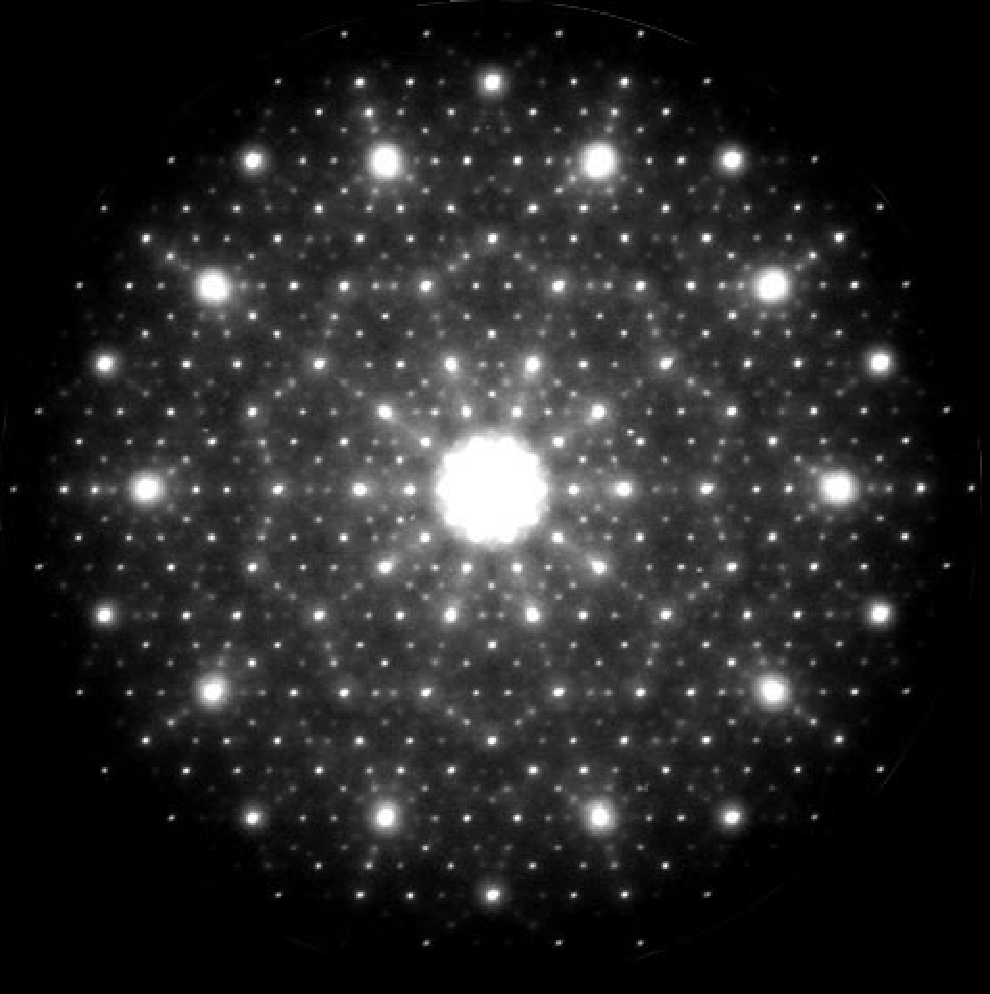
\includegraphics[height = 5cm]{electron-difraction}\hspace*{0.5cm}
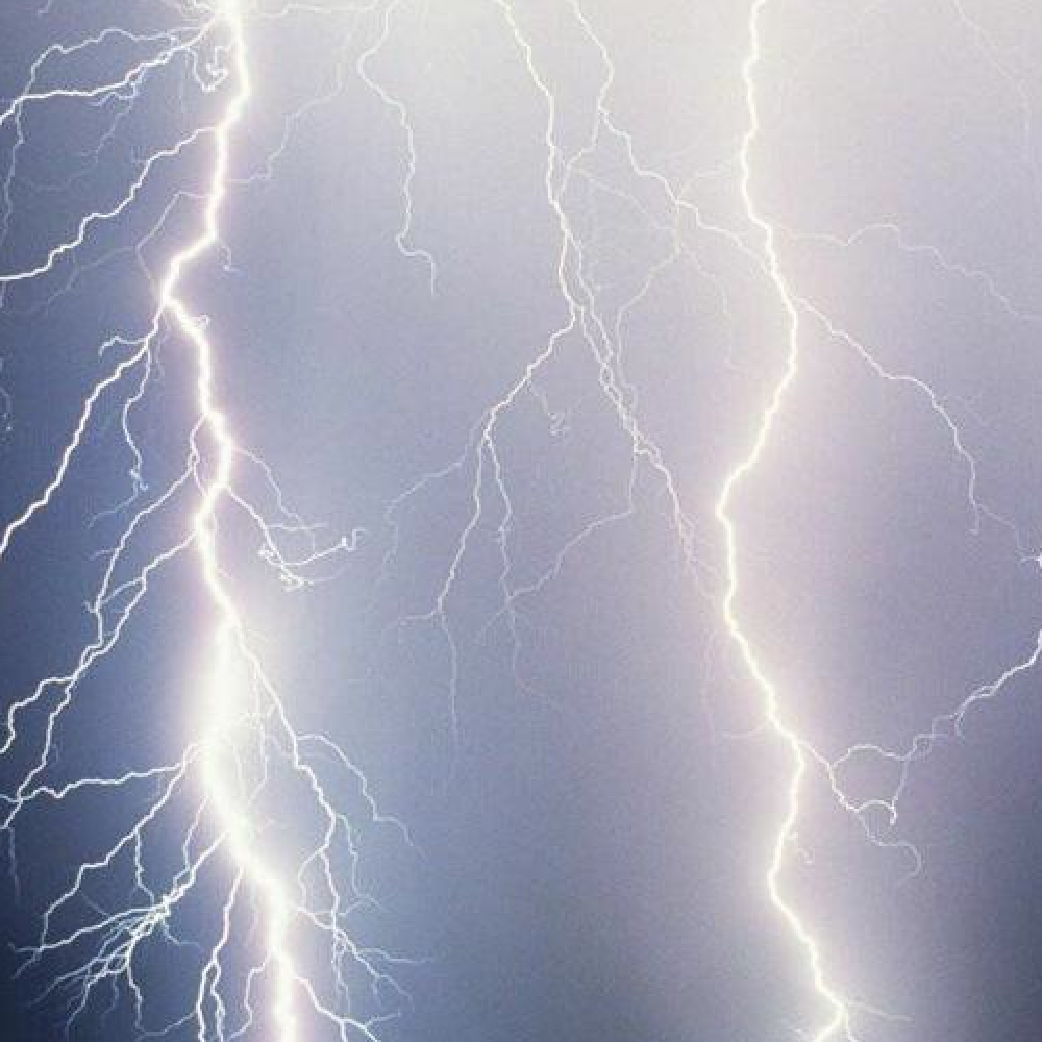
\includegraphics[height = 5cm]{lightning}\hspace*{0.5cm}
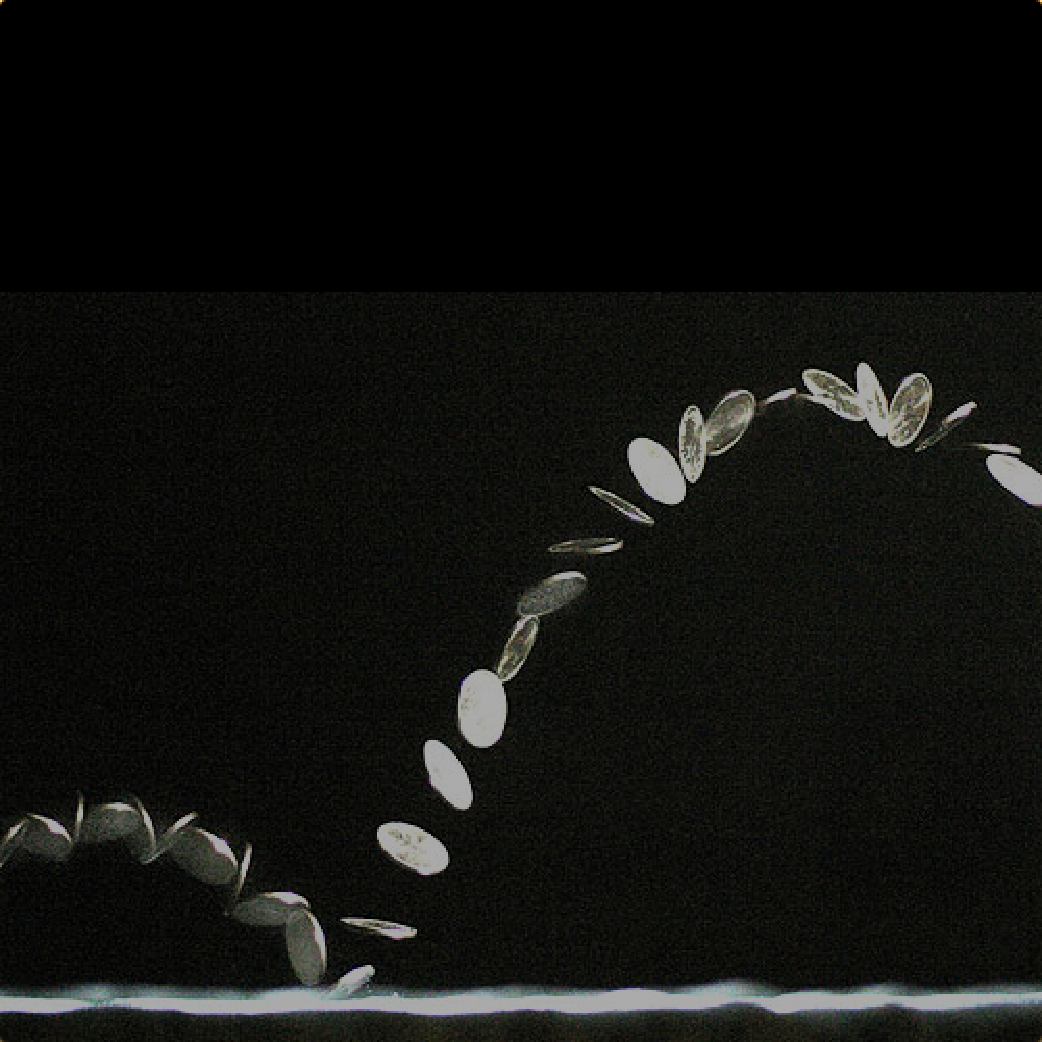
\includegraphics[height = 5cm]{coin-flip}
\end{center}
\vspace*{1cm}

Probability is a measure of uncertainty which can rise in several ways
\begin{triangles}
\item Intrinsic uncertainty in the system 
\item Uncertainty caused by inherent instability of the system
\item Uncertainty caused by lack of knowledge or control over the system
\end{triangles}

\foilhead[-1cm]{Frequentistic interpretation of  probability}

\illustration[height=8cm]{rolling-dice}


Probability is an average occurrence rate in long series of experiments.

\begin{triangles}
\item Law of large numbers
\item Probability is a collective property 
\item Probabilities can be assigned only to future events
\end{triangles}



\foilhead[-1cm]{Bayesian interpretation of probability}


\illustration[height=8cm]{shell-game}
Probability reflects persons individual beliefs on future or unknown events. 

\begin{triangles}
\item Belief updates through the Bayes rule
\item Probability is an inherently subjective property 
\item Probabilities can be assigned  to past, present and future events
\end{triangles}



\foilhead[-1cm]{Ultra-frequentistic interpretation of probability}

\illustration[height=8cm]{pigsfly}

Events with small enough probability do not occur
\begin{triangles}
\item The main tool in classical statistics 
\item Errors in judgement does not matter if a gamma ray pulse kills us.
\item One must avoid the lottery paradox in the reasoning
\end{triangles}


\foilhead[-1cm]{The goal of statistical inference}

\textbf{Frequentist goal}
\begin{triangles}
\item The aim of statistics is to design algorithms that work well on average.
\item For that one needs to specify probabilistic model for data sources.
\item Confidence is the fraction of cases the algorithm works as specified.
\end{triangles}
\vspace*{2cm}

\textbf{Bayesian goal}
\begin{triangles}
\item The aim of statistics is to design algorithms that allow \emph{rational individuals} to reliably update their beliefs through Bayes formula
\item Besides the data source model one has to provide model for initial beliefs.
\item Correctness of an algorithm does not make sense.
\end{triangles}

\middlefoil{Frequentistic methods}

\foilhead[-1cm]{Causation between zero-one events}

Assume that condition A causes the event $B=1$ with probability $p$, i.e.,
\begin{align*}
\pr{B=1|A}=p
\end{align*}
Then the probability is to get $k$ ones in $n$ independent trials is
\begin{align*}
\pr{B_1+\cdots+B_n=k|A}=\binom{n}{k}p^k(1-p)^{n-k}
\end{align*} 
The number of ones in known to have a \emph{binomial distribution}
\begin{align*}
 B_1+\cdots+B_n\sim\mathsf{Bin}(n, p)
\end{align*}

\foilhead[-1cm]{Illustration}

\illustration[width=22cm]{binomial_distribution}
\vspace*{-1cm}

The distribution of  $B_1+\ldots+B_n$ depends solely on the number of trials $n$ and the probability $p$. Some values of $B_1+\ldots+B_n$ are very unlikely.

\foilhead[-1cm]{How to build a statistical test}

\textbf{I. Null hypothesis:}
\begin{triangles}
\item The probability of a single one is $\pr{B_i=1}=p$.
\end{triangles}
\vspace*{1cm}

\textbf{II. Choose value to compute aka test statistic:} 
\begin{triangles}
\item Our test statistic will be $B_1+\ldots+B_n$.
\end{triangles}
\vspace*{1cm}


\textbf{III. Consequences on the observations:} 
\begin{triangles}
\item The observed sum $B_1+\ldots+B_n\sim\mathsf{Bin}(n=20, p=0.5)$.
\item Limit on the tail probability $\pr{|B_1+\ldots+B_n-10|\geq 6}\leq 5\%$
\end{triangles}
\vspace*{1cm}

\textbf{IV. Test procedure}
\begin{triangles}
\item Reject null hypotesis at \emph{significance level} $5\%$ if $|B_1+\ldots+B_n-10|\geq 6$.  
\end{triangles}
 
\foilhead[-1cm]{Properties of statistical tests}

Statistical test is a classification algorithm designed to distinguish a fixed distribution of negative examples specified by a null hypothesis.
\vspace*{2ex}

Any classification algorithm can be converted to a statistical test by finding out the percentage of false positives aka \emph{p-value}:
\begin{triangles}
\item There might exists a closed form solution.
\item We can always estimate p-values using simulations. 
\item Observations must be compressed into a single decision value.
\end{triangles}
\vspace*{2ex}

Testing several hypothesis in parallel increases the number of false positives.  
Several p-value adjustment methods are used to correct the issue:
\begin{triangles}
\item Bonferroni correction is almost optimal 
\item FDR correction controls the expected number false positives  
\end{triangles}  
 

\foilhead[-1cm]{How to build confidence intervals}
 
\textbf{I. Construct a family of statistical tests:}
\begin{triangles}
\item Define a statistical test $T_p$ for all possible parameter values $p$.
\item All tests should share the same test statistic.
\end{triangles}
\vspace*{1cm}

\textbf{II. Perform multiple hypotesis testing for all parameter values:}
\begin{triangles}
\item Accept all parameters values for which pvalue is greather than $\alpha$.  
\item Output a minimal interval that covers all accepted parameter values.
\end{triangles}
\vspace*{1cm}

\textbf{Rationale}
\begin{triangles}
\item The true parameter value is rejected on $\alpha$-fraction of~possible~observations.
\item Otherwise, the true value is inside the predicted interval. 
\end{triangles}


\foilhead[-1cm]{Illustration}
\enlargethispage{0.5cm}
\centerline{
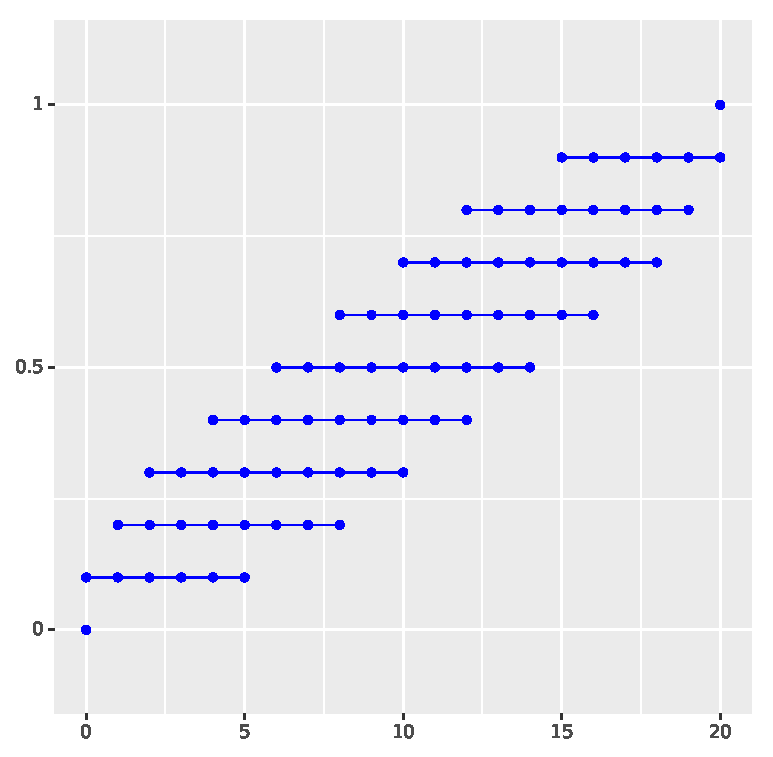
\includegraphics[scale=0.8]{bin_conf_intervals_i}
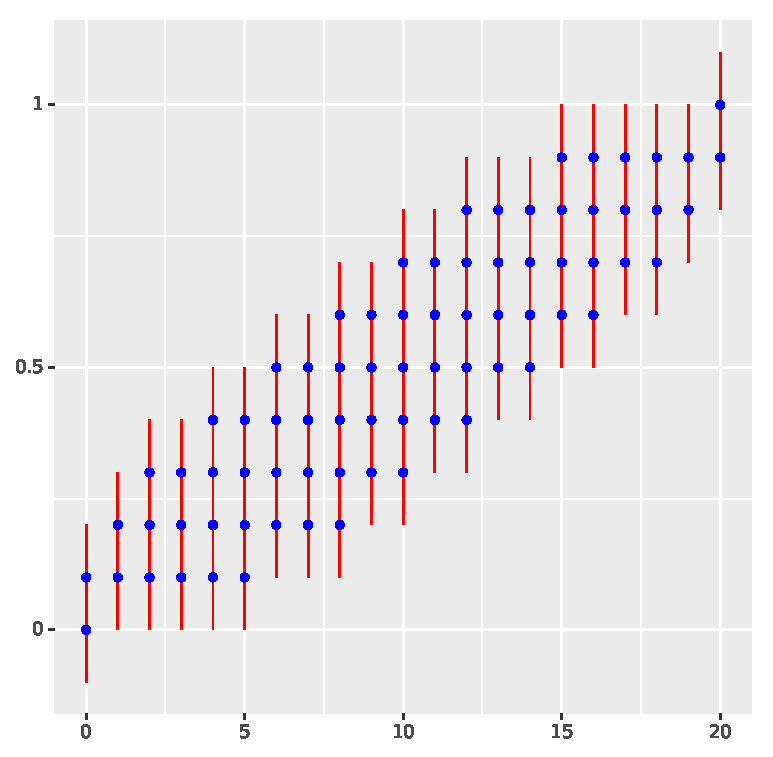
\includegraphics[scale=0.8]{bin_conf_intervals_ii}}
\begin{triangles}
\item Acceptance ranges for different parameter values on the left.
\item Extended parameter ranges covering all accepted parameters on the right.
\item These ranges are the desired confidence intervals.
\end{triangles}


\foilhead[-1cm]{Interpretation of confidence intervals}

\textbf{Definition}
Confidence interval for a parameter $p$ is an outcome of an approximation algorithm. The algorithm  must output an interval $[\hat{p}-\varepsilon,\hat{p}+\varepsilon]$ such that the true estimate is out of this range on $\alpha$  fraction of cases.
\vspace*{2ex}

\textbf{Paradoxical inapplicability}

The definition does not state that the probability $p\in[\hat{p}-\varepsilon,\hat{p}+\varepsilon]$ is $\alpha$!
\begin{triangles}
\item The statement $p\in[\hat{p}-\varepsilon,\hat{p}+\varepsilon]$ is either true or false.
\item There is no probability left. We just \emph{do not know} the answer!
\end{triangles} 
\vspace*{3ex}

\textbf{Ultra-frequentistic resolution}
\begin{triangles}
\item  If $\alpha$ is small enough say $5\%$ then the algorithm is always correct. 
\end{triangles}


\foilhead[-1cm]{Illustrative example}

\illustration[scale=0.8]{confidence_intervals_example}

By increasing the length of the interval we increase the fraction of runs for which the true value of $p$ lies in the interval.


\foilhead[-1cm]{Problems with confidence intervals}

\textbf{Inability to capture background knowledge}
\begin{triangles}
\item What if I know that $p\in[0.1,0.2]$ and observe $B_1=\ldots=B_N=1$?
\item Then the estimate $[\hat{p}-\varepsilon,\hat{p}+\varepsilon]$  is clearly wrong although on average this confidence interval is reasonable.
\end{triangles}
\vspace*{2cm}


\textbf{Multiple hypothesis testing}

\begin{triangles}
\item Using several confidence intervals in parallel increases the fraction of cases where some true estimate is out of the predicted range.
\item We can use p-value adjustment methods are used to correct the issue.
\end{triangles}  


\foilhead[-1cm]{Prediction intervals}

Even if we know the true relation $y=f(\vec{x})$ we cannot predict the observation $y_{i}=f(\vec{x}_i)+\varepsilon_i$, as the noise term $\varepsilon_{i}$ is not known ahead.
\begin{triangles}
\item We cannot give upper and lower bounds for $y_i$ which always hold.
\end{triangles}
\vspace*{4ex}

Instead, we can specify a prediction interval $[y_*-\varepsilon, y_*+\varepsilon]$ so that with probability $95\%$ the resulting measurement $y_i$ is in the range.
\begin{triangles}
\item Usually, the analysis is similar to confidence interval derivation.
\end{triangles}  
\vspace*{4ex}

Interpretation of prediction intervals is different from confidence intervals.

\begin{triangles}
\item The probability estimate holds for the particular interval.
\end{triangles}  

\foilhead[-1cm]{Illustrative example}

\illustration{prediction-intervals-example}

By increasing the length of the prediction interval we increase the fraction of future measurements which fall into interval.



\foilhead[-1cm]{Confidence envelopes}

Confidence intervals is a good way to visualise uncertainty of a particular paramater.
However, we are sometimes interested in the uncertainty many parameters or in the uncertainty of a function:
\begin{triangles}
\item How a predictor $f:[0,1]\to\mathbb{R}$ depends on the training set
\item How a ROC curve $\textsc{Roc}:[0,1]\to[0,1]$ depends on the test set
\item How should a quantile-quantile plot be distributed.
\end{triangles}
\vspace*{4ex}

Confidence bands are generalisations of confidence intervals
\begin{triangles}
\item Pointwise confidence band is a collection of confidence intervals
\item Simultaneous confidence band that encloses $\alpha$-fraction of functions.  
\item Simultaneous confidence bands are much wider than pointwise bands.  
\end{triangles}


\foilhead[-1cm]{Illustrative example}
\enlargethispage{0.5cm}
\centerline{
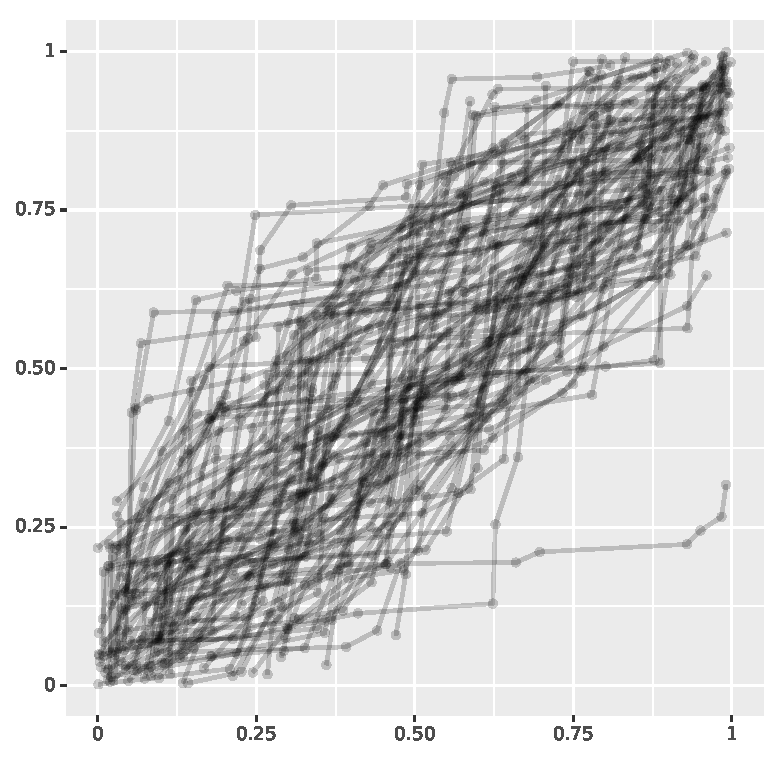
\includegraphics[scale=0.8]{qq_line_distribution}
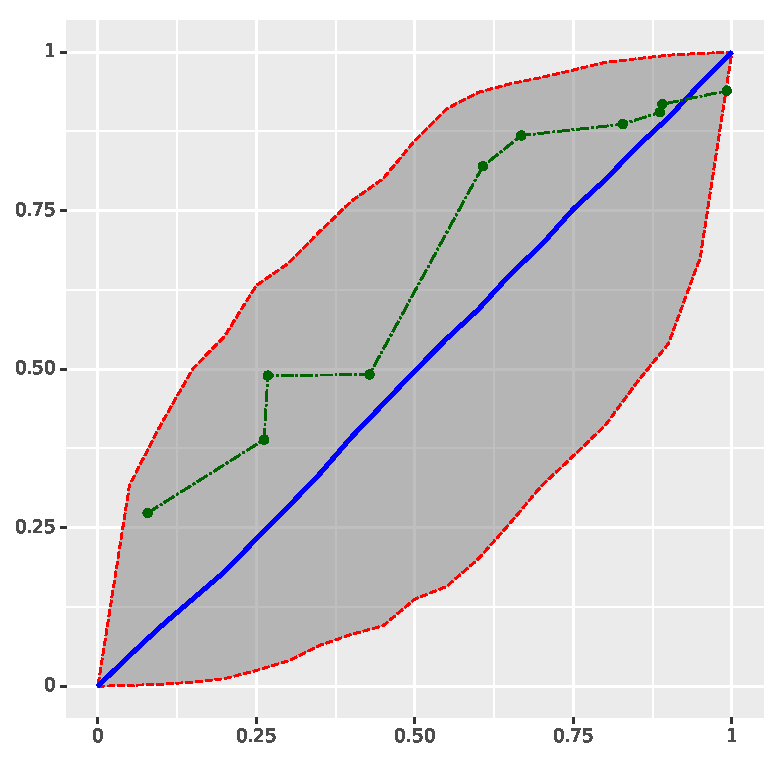
\includegraphics[scale=0.8]{qq_confidence_envelope}}
\begin{triangles}
\item Distribution of qq-lines visualised through a sample on the left.
\item A simulation based pointwise $95\%$ confidence envelope on the right.
\item The significance level that qq-line is inside the envelope is ca $50\%$.
\end{triangles}

\foilhead[-1cm]{Permutation tests}

\textbf{Baseline problem:}
\begin{triangles}
\item Achievable accuracy depends on the data distribution. 
\item Artefacts in the dataset may bias performance measures.
\end{triangles}
\vspace*{2ex}

\textbf{Label permutation.}
A random permutation $\pi$ of outputs $y_i$ destroys correlations between input-output pairs $(\vec{x}_{i}, \vec{y}_{\pi(i)})$ but preserves marginal distribution of inputs and outputs. 
\vspace*{2ex}


\textbf{Permutation test.}
Estimate how probable is to achieve equal or higher accuracy than was observed on the real data.
\begin{triangles}
\item If this probability is small then there must be signal in the data. 
\item The test completely neglect the effect size, i.e., how much results differ.
\item Statistical significance does not imply utility!      
\end{triangles}  



\middlefoil{Bayesian methods}

\foilhead[-0cm]{Bayesian inference procedure}

\illustration[scale=0.9]{bayes-inference}
\vspace*{1cm}
\begin{triangles}
\item Prior distribution $\pr{A}$ encodes the background knowledge
\item The model $\pr{B|A}$  determines how the posterior $\pr{A|B}$ is updated 
\end{triangles}

\foilhead[-1cm]{Posterior of an uninformed person}
\illustration[width=22cm]{uniformed-posterior}
\vspace*{-0.5cm}

With no preferences on the value of $p$ the posterior is strongly skewed towards one and the range $p\in[0.86,1]$
contains $95\%$ of posterior probability.


\foilhead[-1cm]{Posterior of an informed person}
\illustration[width=22cm]{informed-posterior}
\vspace*{-0.5cm}

With the knowledge $p\in[0.1,0.2]$ the posterior is strongly skewed towards $0.2$ and the range $p\in[0.17,0.2]$
contains $95\%$ of posterior probability.



\foilhead[-0cm]{Model behind naive Bayes classifier}

\illustration[scale=0.8]{naive-bayes-scheme}

Underlying class value determines observed attributes 
\begin{triangles}
\item Each attribute $X_i$ is binary 
\item All variables are independent if class is fixed
\item Sometimes we just ignore dependancies for easier modelling
\end{triangles}

\foilhead[-0cm]{Likelihood of the data}

Let us assume that we know the probabilities
\begin{align*}
p_i&=\pr{X_i=1|Class=0}\\
q_i&=\pr{X_i=1|Class=1}
\end{align*}
Then using the independence assumption we get
\begin{align*}
\pr{X_1=a_1,\ldots,X_n=a_n|Class=0}&=\prod_{i=1}^np_i^{a_i}(1-p_i)^{1-a_i}\\
\pr{X_1=a_1,\ldots,X_n=a_n|Class=1}&=\prod_{i=1}^nq_i^{a_i}(1-q_i)^{1-a_i}
\end{align*}

\foilhead[-1cm]{Prior and posterior for the class labels}

\enlargethispage{1.5cm}
Now it is straightforward to derive
\begin{align*}
\pr{Class=0|\vec{X}=\vec{a}}&= \frac{\prod\limits_{i=1}^np_i^{a_i}(1-p_i)^{1-a_i}\cdot\pr{Class=0}}{\pr{\vec{X}=\vec{a}}}\\
\pr{Class=1|\vec{X}=\vec{a}}&= \frac{\prod\limits_{i=1}^nq_i^{a_i}(1-q_i)^{1-a_i}\cdot\pr{Class=1}}{\pr{\vec{X}=\vec{a}}}
\end{align*}
which gives an \emph{odd ratio} 
\begin{align*}
\frac{\pr{Class=0|\vec{X}=\vec{a}}}{\pr{Class=1|\vec{X}=\vec{a}}}&=\frac{\pr{Class=0}}{\pr{Class=1}}\cdot\frac{\prod\limits_{i=1}^np_i^{a_i}(1-p_i)^{1-a_i}}{\prod\limits_{i=1}^nq_i^{a_i}(1-q_i)^{1-a_i}}
\end{align*} 
 
\foilhead[-1cm]{The resulting classifier is a linear classifer}
 
By taking logarithm form the odd ratio we get
\begin{align*}
\log\left(\frac{\pr{Class=0|\vec{X}=\vec{a}}}{\pr{Class=1|\vec{X}=\vec{a}}}\right)&= w_0+\sum_{i=1}^n w_ia_i
\end{align*} 
where 
\begin{align*}
w_0&=\log\left(\frac{\pr{Class=0}}{\pr{Class=1}}\right)+\sum_{i=1}^n\log\left(\frac{1-p_i}{1-q_i}\right)\\
w_i&=\log \left(\frac{p_i}{1-p_i}\cdot\frac{1-q_i}{q_i}\right) 
\end{align*}

\foilhead[-1cm]{How to train the classifier?}
A frequentistic approach is to fix probabilities from the training sample
\begin{align*}
p_i&=\frac{\#\set{\text{data points form class 0 with $X_i=1$}}}{\#\set{\text{data points form class 0}}}\\
q_i&=\frac{\#\set{\text{data points form class 1 with $X_i=1$}}}{\#\set{\text{data points form class 1}}}
\end{align*}
However if some value does not occur for $X_i$ in the training sample we get overly confident results. Thus, Bayesian mean estimate is better alternative  
\begin{align*}
p_i&=\frac{\#\set{\text{data points form class 0 with $X_i=1$}}+1}{\#\set{\text{data points form class 0}}+2}\\
q_i&=\frac{\#\set{\text{data points form class 1 with $X_i=1$}}+1}{\#\set{\text{data points form class 1}}+2}
\end{align*}

\foilhead[-1cm]{Going beyond naive Bayesian models}
\illustration[scale=0.8]{bayesian-network}

Complex causal models are often defined through Bayesian networks
\begin{triangles}
\item A complex processes is first split into sub-events
\item Direct causal dependencies between sub-events are detected
\item Causation mechanisms are characterised with probability tables
\end{triangles} 
  
\foilhead[-1cm]{Strength and weaknesses of Bayesian networks}

\textbf{Strengths}
\begin{triangles}
\item Bayesian networks are easy to interpret
\item Bayesian networks are good for formalising fuzzy background knowledge
\item Estimation of individual probability tables is tractable
\item There are tools for doing inference with Bayesian networks  
\end{triangles}
\vspace*{1cm}

\textbf{Weaknesses}
\begin{triangles}
\item You must know the causal structure of sub-events  
\item Identification of causal structure form data alone is very difficult
\item It is notoriously difficult to model non-trivial causal dependencies
\item Standard inference procedures often do not have closed solutions 
\end{triangles}

\end{document}
